\begin{enumerate}[label=\thesection.\arabic*.,ref=\thesection.\theenumi]
\numberwithin{equation}{enumi}
\item
Sketch the Polar Plot of
\begin{align}
G\brak{s} = \frac{1}{s\brak{1+s^{2}}}
\label{eq:ee18btech11023_gain}
\end{align}
\\
\solution  From \label{eq:ee18btech11023_gain},

\begin{align}
G\brak{\j\omega} &=   \frac{1}{\j\omega\brak{1-{\omega}^{2}}}
\\
      \abs{G\brak{\j\omega}} &= \frac{1}{\abs{\omega\brak{1-{\omega}^{2}}}}
\\
    \angle G\brak{\j\omega} &= 
\begin{cases}
\frac{\pi}{2} & \omega > 1
\\
-\frac{\pi}{2} & 0 < \omega < 1
\end{cases}
    \end{align}
%
The corresponding polar plot is generated in Fig.   \ref{fig:ee18btech11023} using 
\begin{lstlisting}
codes/ee18btech11023.py
\end{lstlisting}

\begin{figure}[!ht]
\centering
  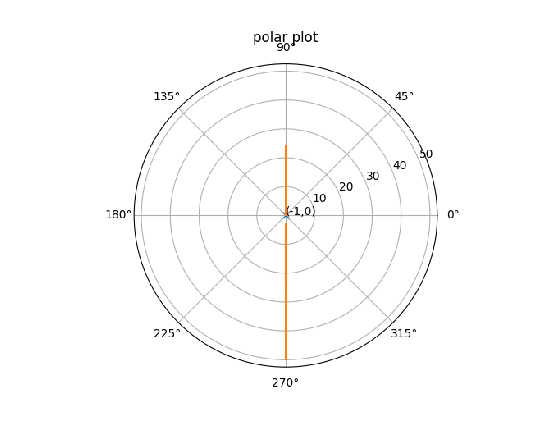
\includegraphics[width=\columnwidth]{./figs/ee18btech11023/ee18btech11023_1c.eps}
  \caption{}
  \label{fig:ee18btech11023}
\end{figure}


\item
 Stability

\break for the given transfer function 
\begin{align}
    G\brak{s} = \frac{1}{s\brak{1+s^{2}}}
\end{align}
The polar plots use open loop transfer function, hence the reference point for determining
stability is shifted to (–1, 0)
\center
 If (–1,0) is exactly on the polar plot then the system is marginally stable
polar plot useful to find the stability of given transfer function
from the graph we can see that (-1,0) is lying exactly on polar plot


\center so the system is marginally stable
\end{enumerate}
